\documentclass{standalone}

\usepackage{tikz}
\usepackage{tkz-euclide}
\usetikzlibrary{calc}
\usetikzlibrary{positioning}
\usetikzlibrary{arrows.meta}

\usepackage{times}


\begin{document}
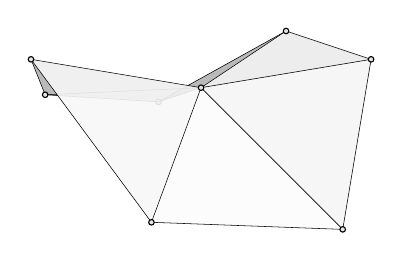
\begin{tikzpicture}[%
  >={Stealth[scale=1.0]},
  scale=1.8
]

  \tkzDefPoint(0.0, 0.0){x}

  \tkzDefPoint(1.0, -1.0){A}
  \tkzDefPoint(1.2, 0.2){B}
  \tkzDefPoint(0.6, 0.4){C}
  \tkzDefPoint(-0.3, -0.1){D}
  \tkzDefPoint(-1.1, -0.05){E}
  \tkzDefPoint(-1.2, 0.2){F}
  \tkzDefPoint(-0.35, -0.95){G}

  \tkzFillPolygon[color=black!90,opacity=0.3](x,C,D)
  \tkzDrawSegments(C,D)
  \tkzFillPolygon[color=black!90,opacity=0.3](x,D,E)
  \tkzDrawPoints(D)
  \tkzDrawSegments(x,D x,E D,E)

  \tkzFillPolygon[color=black!90,opacity=0.3](x,E,F)

  \tkzFillPolygon[color=black!4,opacity=0.9](x,A,B)
  \tkzFillPolygon[color=black!8,opacity=0.9](x,B,C)
  \tkzFillPolygon[color=black!3,opacity=0.9](x,F,G)
  \tkzFillPolygon[color=black!1,opacity=0.9](x,G,A)

  \tkzDrawSegments(x,A x,B x,C x,F x,G)
  \tkzDrawSegments(A,B B,C E,F F,G G,A)

  \tkzDrawPoints(x,A,B,C,E,F,G)

\end{tikzpicture}
\end{document}
